% !TEX program = xelatex
% ------------------------------------------------------------
% Open-source Beamer Template
% Version: 1.0
% Recommended compiler: XeLaTeX
%
% A clean Beamer template for academic presentations.
% ------------------------------------------------------------

\documentclass[10pt,aspectratio=169]{beamer}

% ---------------- Packages ----------------
\usepackage[fontset=none]{ctex}
\usepackage{fontspec}
\usepackage{amsmath,amssymb,bm,mathtools}
\usepackage{booktabs,array,tabularx,multirow}
\usepackage{graphicx}
\usepackage{xcolor}
\usepackage{tikz}
\usepackage{adjustbox}
\usepackage{hyperref}

\usetikzlibrary{arrows.meta,positioning,calc}
\graphicspath{{figure/}}

% ---------------- Theme ----------------
% Metropolis is used mainly for the title page and section pages.
\usetheme[numbering=fraction,progressbar=none,sectionpage=progressbar]{metropolis}
\metroset{
  titleformat=regular,
  titleformat title=regular,
  titleformat subtitle=regular,
  titleformat section=regular,
  titleformat frame=regular
}

% ---------------- Fonts ----------------
% English font fallback
\IfFontExistsTF{Times New Roman}
  {\setmainfont{Times New Roman}\setsansfont{Times New Roman}}
  {\setmainfont{Noto Serif}\setsansfont{Noto Sans}}

% Chinese font fallback
\IfFontExistsTF{Kaiti SC}
  {\setCJKmainfont[AutoFakeBold=2.5]{Kaiti SC}
   \setCJKsansfont[AutoFakeBold=2.5]{Kaiti SC}}
  {\IfFontExistsTF{Noto Serif CJK SC}
    {\setCJKmainfont[AutoFakeBold=2.5]{Noto Serif CJK SC}
     \setCJKsansfont[AutoFakeBold=2.5]{Noto Serif CJK SC}}
    {\setCJKmainfont[AutoFakeBold=2.5]{AR PL UMing CN}
     \setCJKsansfont[AutoFakeBold=2.5]{AR PL UMing CN}}}

% ---------------- Colors ----------------
\definecolor{textred}{RGB}{125,34,51}
\definecolor{deepred}{RGB}{125,34,51}
\definecolor{darkred}{RGB}{92,12,20}
\definecolor{ink}{RGB}{20,20,20}
\definecolor{warmgray}{RGB}{92,88,84}
\definecolor{linegray}{RGB}{208,208,208}
\definecolor{footgray}{RGB}{228,228,228}
\definecolor{gold}{RGB}{180,130,40}

\setbeamercolor{palette primary}{fg=white,bg=deepred}
\setbeamercolor{title separator}{fg=textred}
\setbeamercolor{progress bar}{fg=deepred,bg=linegray}
\setbeamercolor{progress bar in section page}{fg=textred,bg=linegray}
\setbeamercolor{normal text}{fg=ink,bg=white}
\setbeamercolor{structure}{fg=deepred}
\setbeamercolor{alerted text}{fg=deepred}
\setbeamercolor{title}{fg=ink,bg=white}

% ---------------- Layout ----------------
\setbeamertemplate{navigation symbols}{}
\setbeamersize{text margin left=0.82cm,text margin right=0.82cm}
\setbeamerfont{normal text}{size=\fontsize{9.2}{13}\selectfont}
\setbeamerfont{frametitle}{size=\fontsize{15}{17}\selectfont,series=\mdseries}
\setbeamertemplate{itemize item}{\color{deepred}$\bullet$}
\setbeamertemplate{itemize subitem}{\color{textred}$\circ$}
\setlength{\tabcolsep}{3pt}
\linespread{1.02}

% ---------------- Frame title with progress line ----------------
\makeatletter
\setbeamertemplate{frametitle}{%
  \ifx\insertframetitle\@empty
  \else
    \nointerlineskip
    \vspace*{0.23cm}%
    \hspace*{-0.82cm}% offset left text margin
    \begin{tikzpicture}
      \pgfmathsetmacro{\progress}{\insertframenumber/\inserttotalframenumber}
      \node[
        anchor=west,
        inner sep=0pt,
        text=black,
        font=\fontsize{11}{11}\bfseries\selectfont
      ] at (0.75cm, 0.35cm) {\strut\insertframetitle};
      \draw[linegray, line width=0.6pt] (0, 0) -- (\paperwidth, 0);
      \draw[textred, line width=0.6pt] (0, 0) -- ({\progress*\paperwidth}, 0);
    \end{tikzpicture}
    \vspace{-0.02cm}
  \fi
}
\makeatother

% ---------------- Footer ----------------
% Replace the three placeholders below with short public information.
% To remove the footer entirely, use: \setbeamertemplate{footline}{}
\setbeamercolor{footleft}{fg=white,bg=darkred}
\setbeamercolor{footmid}{fg=deepred,bg=footgray}
\setbeamercolor{footright}{fg=deepred,bg=white}

\newcommand{\footerleft}{Short Author / Topic}
\newcommand{\footermid}{Short Deck Title}
\newcommand{\footerright}{Venue / Year}

\setbeamertemplate{footline}{%
  \leavevmode%
  \hbox{%
    \begin{beamercolorbox}[wd=0.30\paperwidth,ht=0.30cm,dp=0.06cm,center]{footleft}
      \raisebox{0.03cm}{\fontsize{7}{8}\selectfont \footerleft}
    \end{beamercolorbox}%
    \begin{beamercolorbox}[wd=0.50\paperwidth,ht=0.30cm,dp=0.06cm,center]{footmid}
      \raisebox{0.03cm}{\fontsize{7}{8}\selectfont \footermid}
    \end{beamercolorbox}%
    \begin{beamercolorbox}[wd=0.20\paperwidth,ht=0.30cm,dp=0.06cm,center]{footright}
      \raisebox{0.03cm}{\fontsize{7}{8}\selectfont \footerright\quad \insertframenumber/\inserttotalframenumber}
    \end{beamercolorbox}%
  }%
}

% ---------------- Reusable commands ----------------
\newenvironment{tightitemize}{%
  \begin{itemize}
  \setlength{\itemsep}{0.12em}
  \setlength{\parskip}{0pt}
}{\end{itemize}}

\newcommand{\hl}[1]{\textcolor{deepred}{#1}}
\newcommand{\subhead}[1]{\vspace{0.25em}{\fontsize{9.2}{13}\selectfont\color{deepred}\bfseries #1}\par\vspace{0.08em}}
\newcommand{\smallgray}[1]{{\fontsize{9.2}{13}\selectfont\color{ink}#1}}
\newcommand{\fig}[2][]{\includegraphics[#1]{#2}}
\newcommand{\source}[1]{{\vspace{0.08em}\fontsize{6.5}{8}\selectfont\color{warmgray}Source: #1\par}}
\newcommand{\eqnote}[1]{\vspace{-0.10em}{\fontsize{9.2}{13}\selectfont\color{ink}#1\par\vspace{0.34em}}}
\newcommand{\formulanote}[1]{{\fontsize{9.2}{13}\selectfont\hspace{2em}#1\par\vspace{0.12em}}}

\newenvironment{slidebody}{%
  \fontsize{9.2}{13}\selectfont
  \setlength{\abovedisplayskip}{0.30em}%
  \setlength{\belowdisplayskip}{0.30em}%
  \setlength{\abovedisplayshortskip}{0.18em}%
  \setlength{\belowdisplayshortskip}{0.18em}%
}{ }

% ---------------- Title information ----------------
\title{Main Title}
\subtitle{\textbf{Subtitle or Paper Title}}
\author{{\fontsize{9.2}{13}\selectfont Author / Presenter}}
\date{}
\institute{{\fontsize{9.2}{13}\selectfont Institution or Event\\[0.18cm]Month Year}}

% ---------------- Section transition page ----------------
\setbeamertemplate{section page}{
  \centering
  \begin{minipage}{22em}
    \centering
    \usebeamercolor[fg]{section title}
    \usebeamerfont{section title}
    \insertsectionhead\\[-1ex]
    \usebeamertemplate*{progress bar in section page}
    \par
  \end{minipage}
  \par
  \vspace{\baselineskip}
}

\AtBeginSection[]{%
  \begin{frame}[plain,c,noframenumbering]
    \sectionpage
  \end{frame}
}

% ============================================================
% Document starts here
% ============================================================
\begin{document}

\maketitle

\section{Motivation}

\begin{frame}[t]{Motivation}
\vspace{-0.42cm}
\subhead{Research background}
{\fontsize{9.2}{13}\selectfont
\hspace{2em} Use this line to briefly introduce the general research area and its importance.

\begin{tightitemize}
  \item \hl{\textbf{Fact 1:}} Key empirical or institutional background.
  \item \hl{\textbf{Fact 2:}} Important theoretical or policy gap.
  \item \hl{\textbf{Question:}} Your central research question.
\end{tightitemize}}
\end{frame}

\section{Framework}

\begin{frame}[t]{Model Setup}
\vspace{-0.62cm}
\begin{slidebody}
\subhead{Core equation}
\vspace{-0.45cm}
\[
Y_{it}=\alpha+\beta X_{it}+\gamma_i+\lambda_t+\varepsilon_{it}
\]
\formulanote{Use this line to explain the economic meaning of the equation and the identification logic.}

\subhead{Interpretation}
\vspace{-0.20cm}
\begin{tightitemize}
  \item Explain the dependent variable.
  \item Explain the treatment or key explanatory variable.
  \item Explain the fixed effects or controls.
\end{tightitemize}
\end{slidebody}
\end{frame}

\section{Results}

\begin{frame}[t]{Figure or Table Layout}
\vspace{-0.72cm}
\subhead{Main result}
{\fontsize{9.2}{13}\selectfont
\begin{columns}[T,totalwidth=\textwidth]
\begin{column}{0.58\textwidth}
\begin{center}
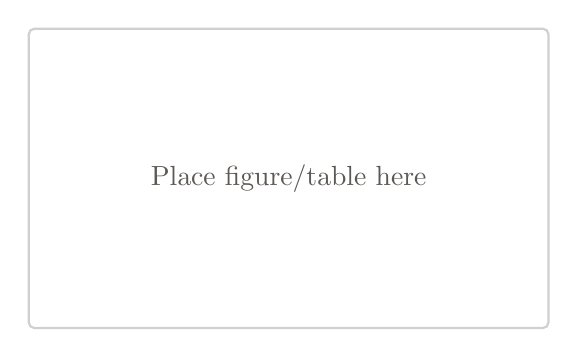
\begin{tikzpicture}
  \draw[linegray, line width=0.8pt, rounded corners=2pt] (0,0) rectangle (6.6,3.8);
  \node[text=warmgray] at (3.3,1.9) {Place figure/table here};
\end{tikzpicture}
\end{center}
% Example for real figure:
% \fig[width=\linewidth,height=0.66\textheight,keepaspectratio]{figure_name.png}
\end{column}
\begin{column}{0.40\textwidth}
\subhead{Takeaways}
\begin{tightitemize}
  \item Result 1.
  \item Result 2.
  \item Mechanism or interpretation.
\end{tightitemize}
\end{column}
\end{columns}}
\end{frame}

\begin{frame}[t]{Summary Table}
\vspace{-0.40cm}
\vfill
\begin{center}
\begin{minipage}{0.86\textwidth}
{\color{black}
\renewcommand{\arraystretch}{1.25}
\setlength{\tabcolsep}{7pt}
\fontsize{9.2}{13}\selectfont
\begin{tabularx}{\textwidth}{>{\centering\arraybackslash}m{0.24\textwidth}>{\raggedright\arraybackslash}X}
\toprule[0.9pt]
\textbf{Item} & \textbf{Description} \\
\midrule
Research question & Your question \\
\addlinespace[0.12cm]
Method & Your method \\
\addlinespace[0.12cm]
Main result & Your core result \\
\addlinespace[0.12cm]
Contribution & Your contribution \\
\bottomrule[0.9pt]
\end{tabularx}}
\end{minipage}
\end{center}
\vfill
\end{frame}

\section{Conclusion}

\begin{frame}[t]{Conclusion}
\vspace{-0.42cm}
\subhead{Main messages}
{\fontsize{9.2}{13}\selectfont
\begin{tightitemize}
  \item \textbf{Message 1:} One-sentence conclusion.
  \item \textbf{Message 2:} One-sentence implication.
  \item \textbf{Message 3:} One-sentence limitation or extension.
\end{tightitemize}}
\end{frame}

\section{Thanks}

\end{document}

